%%%%%%%%%%%%%%%%%%%%%%%%%%%%%%%%%%%%%%%%%%%%%%%%%%%%%%%%%%%%%%%%%%%%
\section{Overview}
\label{sec:fdsp-apa-intro}

Anode planes (or wire planes) are the far detector elements used to sense, through both signal induction and direct collection, the ionization electrons that are created when charged particles traverse the liquid argon volume inside the single-phase LArTPC. To facilitate fabrication and installation underground, the anode design is modular, with anode plane assemblies (APAs) tiled together to form the readout system for a \SI{10}{kton} detector. A single APA is \SI{6}{m} high by \SI{2.3}{m} wide, but two of them are connected vertically, and twenty-five of these vertical stacks are linked together to define a \SI{12}{m} tall by \SI{58}{m} long mostly-active readout plane.  As described below, the planes are active on both sides, so three such wire readout planes are interleaved with two high voltage surfaces to define four \SI{3.6}{m} wide drift regions inside each DUNE far detector module, as shown in the detector schematic views in Figure~\ref{fig:FarDet-interior}.  Each single-phase \SI{10}{kton} module, therefore, will contain 150 anode plane assemblies.

\begin{dunefigure}[Schematic view of a DUNE \SI{10}{kton} single phase TPC module]{fig:FarDet-interior}
{Left: End-on schematic view of the active argon volume showing the four drift regions and anode-cathode plane ordering of the TPC inside the detector. Right: View of the partially installed DUNE TPC inside the membrane cryostat. The APAs are shown in red, CPAs are in cyan, field-cage modules in yellow/green.  Some of the field-cage modules are in their folded position against the cathode to providing aisle access during installation.}
\setlength{\fboxsep}{0pt}
\setlength{\fboxrule}{0.5pt}
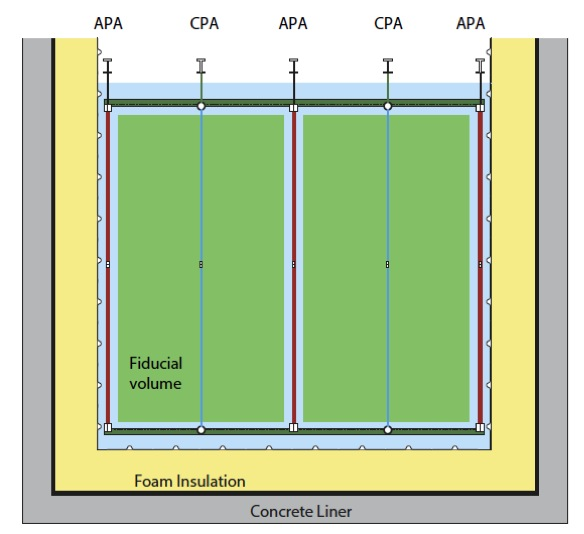
\includegraphics[width=0.445\textwidth, trim=0mm 3.7mm 0mm 0mm, clip]{apa-dune-sp-endview.jpg}\hspace{0.01\textwidth}
\fbox{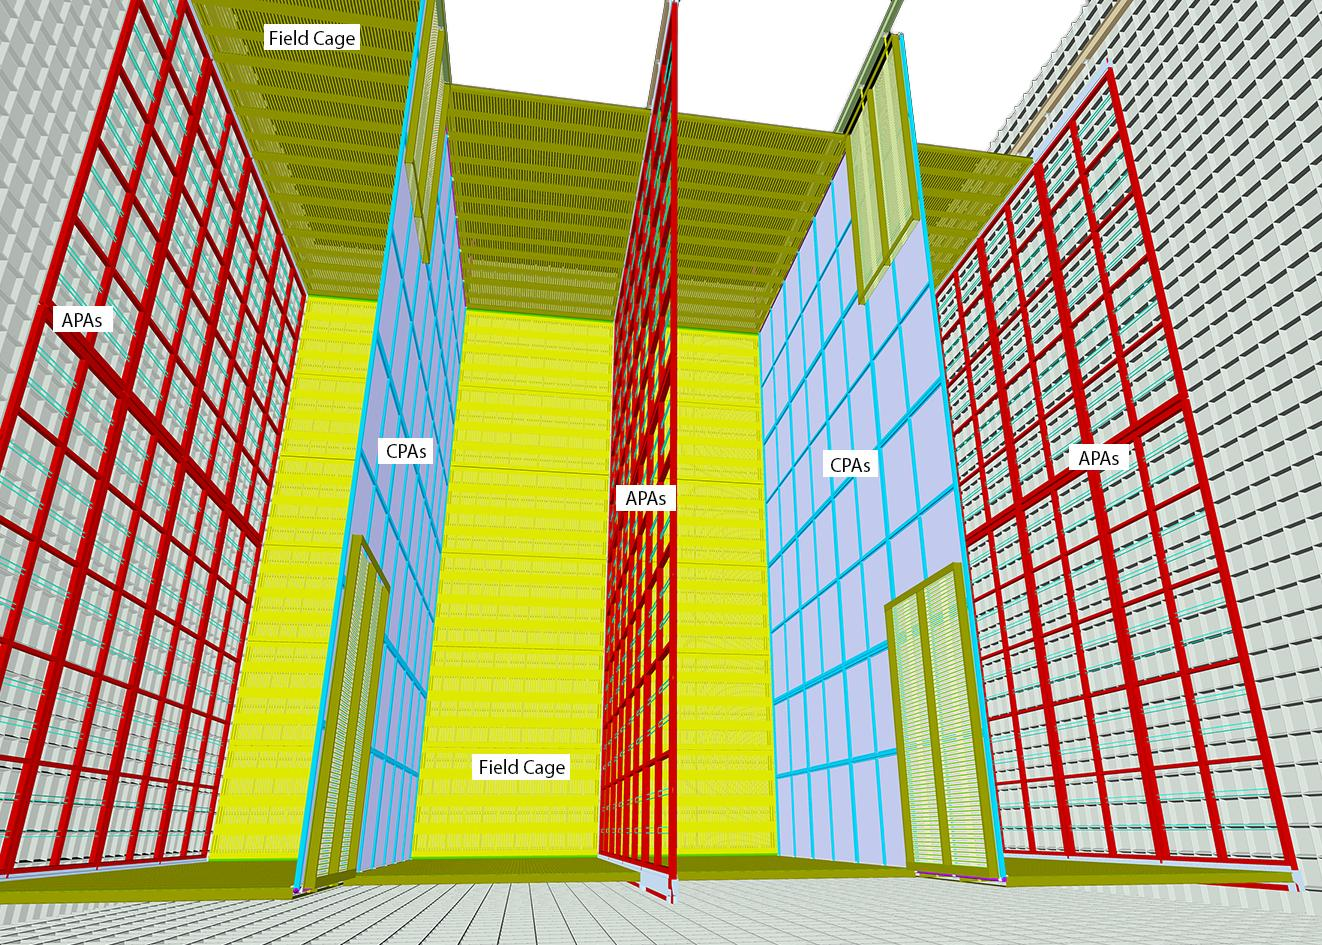
\includegraphics[width=0.52\textwidth]{apa-dune-sp-floor-view.jpg}}
\end{dunefigure}

Each APA frame is covered by over 2,500 sense wires laid in three planes that are oriented at angles to each other (a vertical collection plane, $X$, and two induction planes at $\pm35.7^\circ$ to the vertical, $U$ and $V$) to provide multi-dimensional reconstruction of particle tracks.  An additional 960 wires that are not read out make up an outer shielding plane, $G$, to improve signal shapes on the $U$ induction channels.  The angled wires are wrapped around the frame from one side to the other, allowing all channels to be read out from one end of the APA only (the top or bottom), and thereby minimizing the dead regions between neighboring APAs. Signals induced or collected on the wires are transferred through soldered connections to wire termination boards mounted at the end of the APA frame that in-turn connect to front-end readout electronics sitting in the argon.  Figures~\ref{fig:tpc_apa1} and \ref{fig:tpc_apa2} illustrate the layout of the wires on an APA, showing how they wrap around the frame and terminate on wire boards at the head end where readout electronics are mounted.

The APAs represent a critical interface point between the various detector sub-systems within the DUNE single-phase TPC.  As already mentioned, the TPC readout electronics mount directly to the APA frames.  Photon detectors for detecting scintillation light produced in the argon are also housed inside the frames, sandwiched between the wires on the two sides, requiring careful coordination in the frame design as well as placing a requirement on the transparency of the APA structures.  In addition, the electric field cage panels connect directly to the edges of the APA frames.  Finally, the APAs must support the routing of cables for both the TPC electronics and the photon detector systems. All of these considerations have important impacts on the design, fabrication, and installation planning for the DUNE APAs.   

\begin{dunefigure}[Illustration of the APA wire layout]{fig:tpc_apa1}
{Illustration of the DUNE APA wire wrapping scheme showing small portions of the wires from the three signal planes ($U,V,X$). The fourth wire plane ($G$) above these three, and parallel to $X$, is present to improve the pulse shape on the $U$ plane signals. The TPC electronics boxes, shown in blue on the right, mount directly to the frame and process signals from both the collection and induction channels. The APA is shown turned on its side in a horizontal orientation.} 
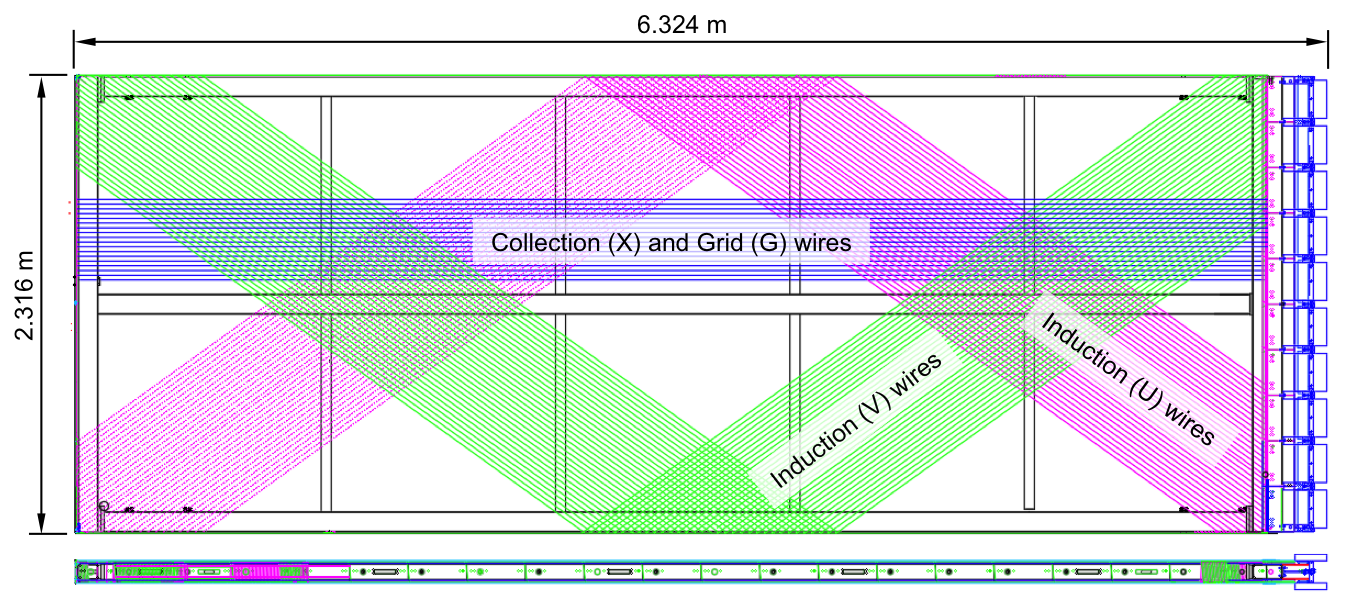
\includegraphics[width=\textwidth]{apa-drawing-wire-configuration.png} 
\end{dunefigure} 

\begin{dunefigure}[Cross-section view of the head end and wire layers of an APA]{fig:tpc_apa2}
{Cross-section view of an APA frame near the head end showing the layers of wires ($X,V,U,G$ inside to out) on both sides of the frame and terminating on wire boards at the head end of the frame, which connect directly to TPC readout electronics.} 
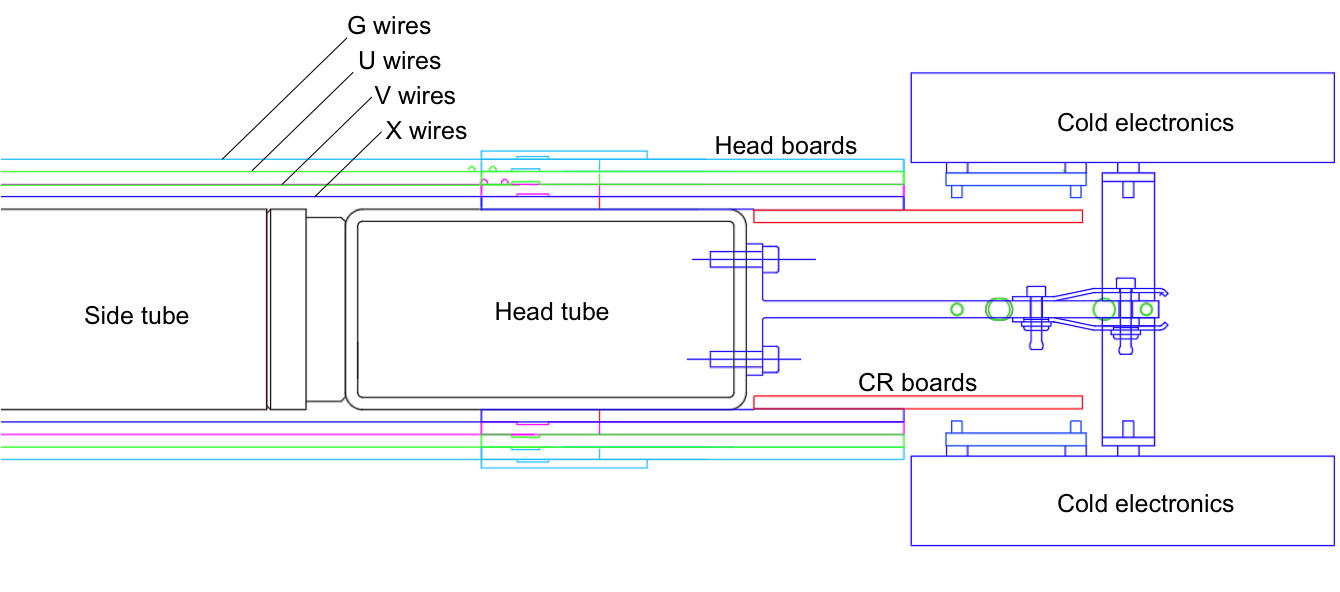
\includegraphics[width=0.95\textwidth]{apa-drawing-cross-section.png} 
\end{dunefigure} 

Full-scale APAs have recently been produced at the Physical Sciences Laboratory (PSL) at the University of Wisconsin as well as at the Daresbury Laboratory in the UK for the ProtoDUNE project at CERN. Figure~\ref{fig:apa-photo} shows a completed APA produced at PSL just before shipment to CERN for use in ProtoDUNE. This effort has greatly informed the design and production planning for the DUNE far detectors, and future ProtoDUNE running is expected to provide valuable validation information for many fundamental aspects of the DUNE APA design. 

The design, construction, testing, and installation of the DUNE APAs is overseen by the APA Consortium within the DUNE Collaboration. Multiple APA production sites will be set up in the US and the UK, with each nation producing approximately half of the APAs needed for the DUNE single-phase detectors.  Factory setup is anticipated to begin in 2020, with APA fabrication for the first \SI{10}{kton} far detector module running from 2021--2023.  

\begin{dunefigure}[Photo of a completed ProtoDUNE APA.]{fig:apa-photo}
{Completed ProtoDUNE APA ready for shipment to CERN.}
\setlength{\fboxsep}{0pt}
\setlength{\fboxrule}{0.5pt}
\fbox{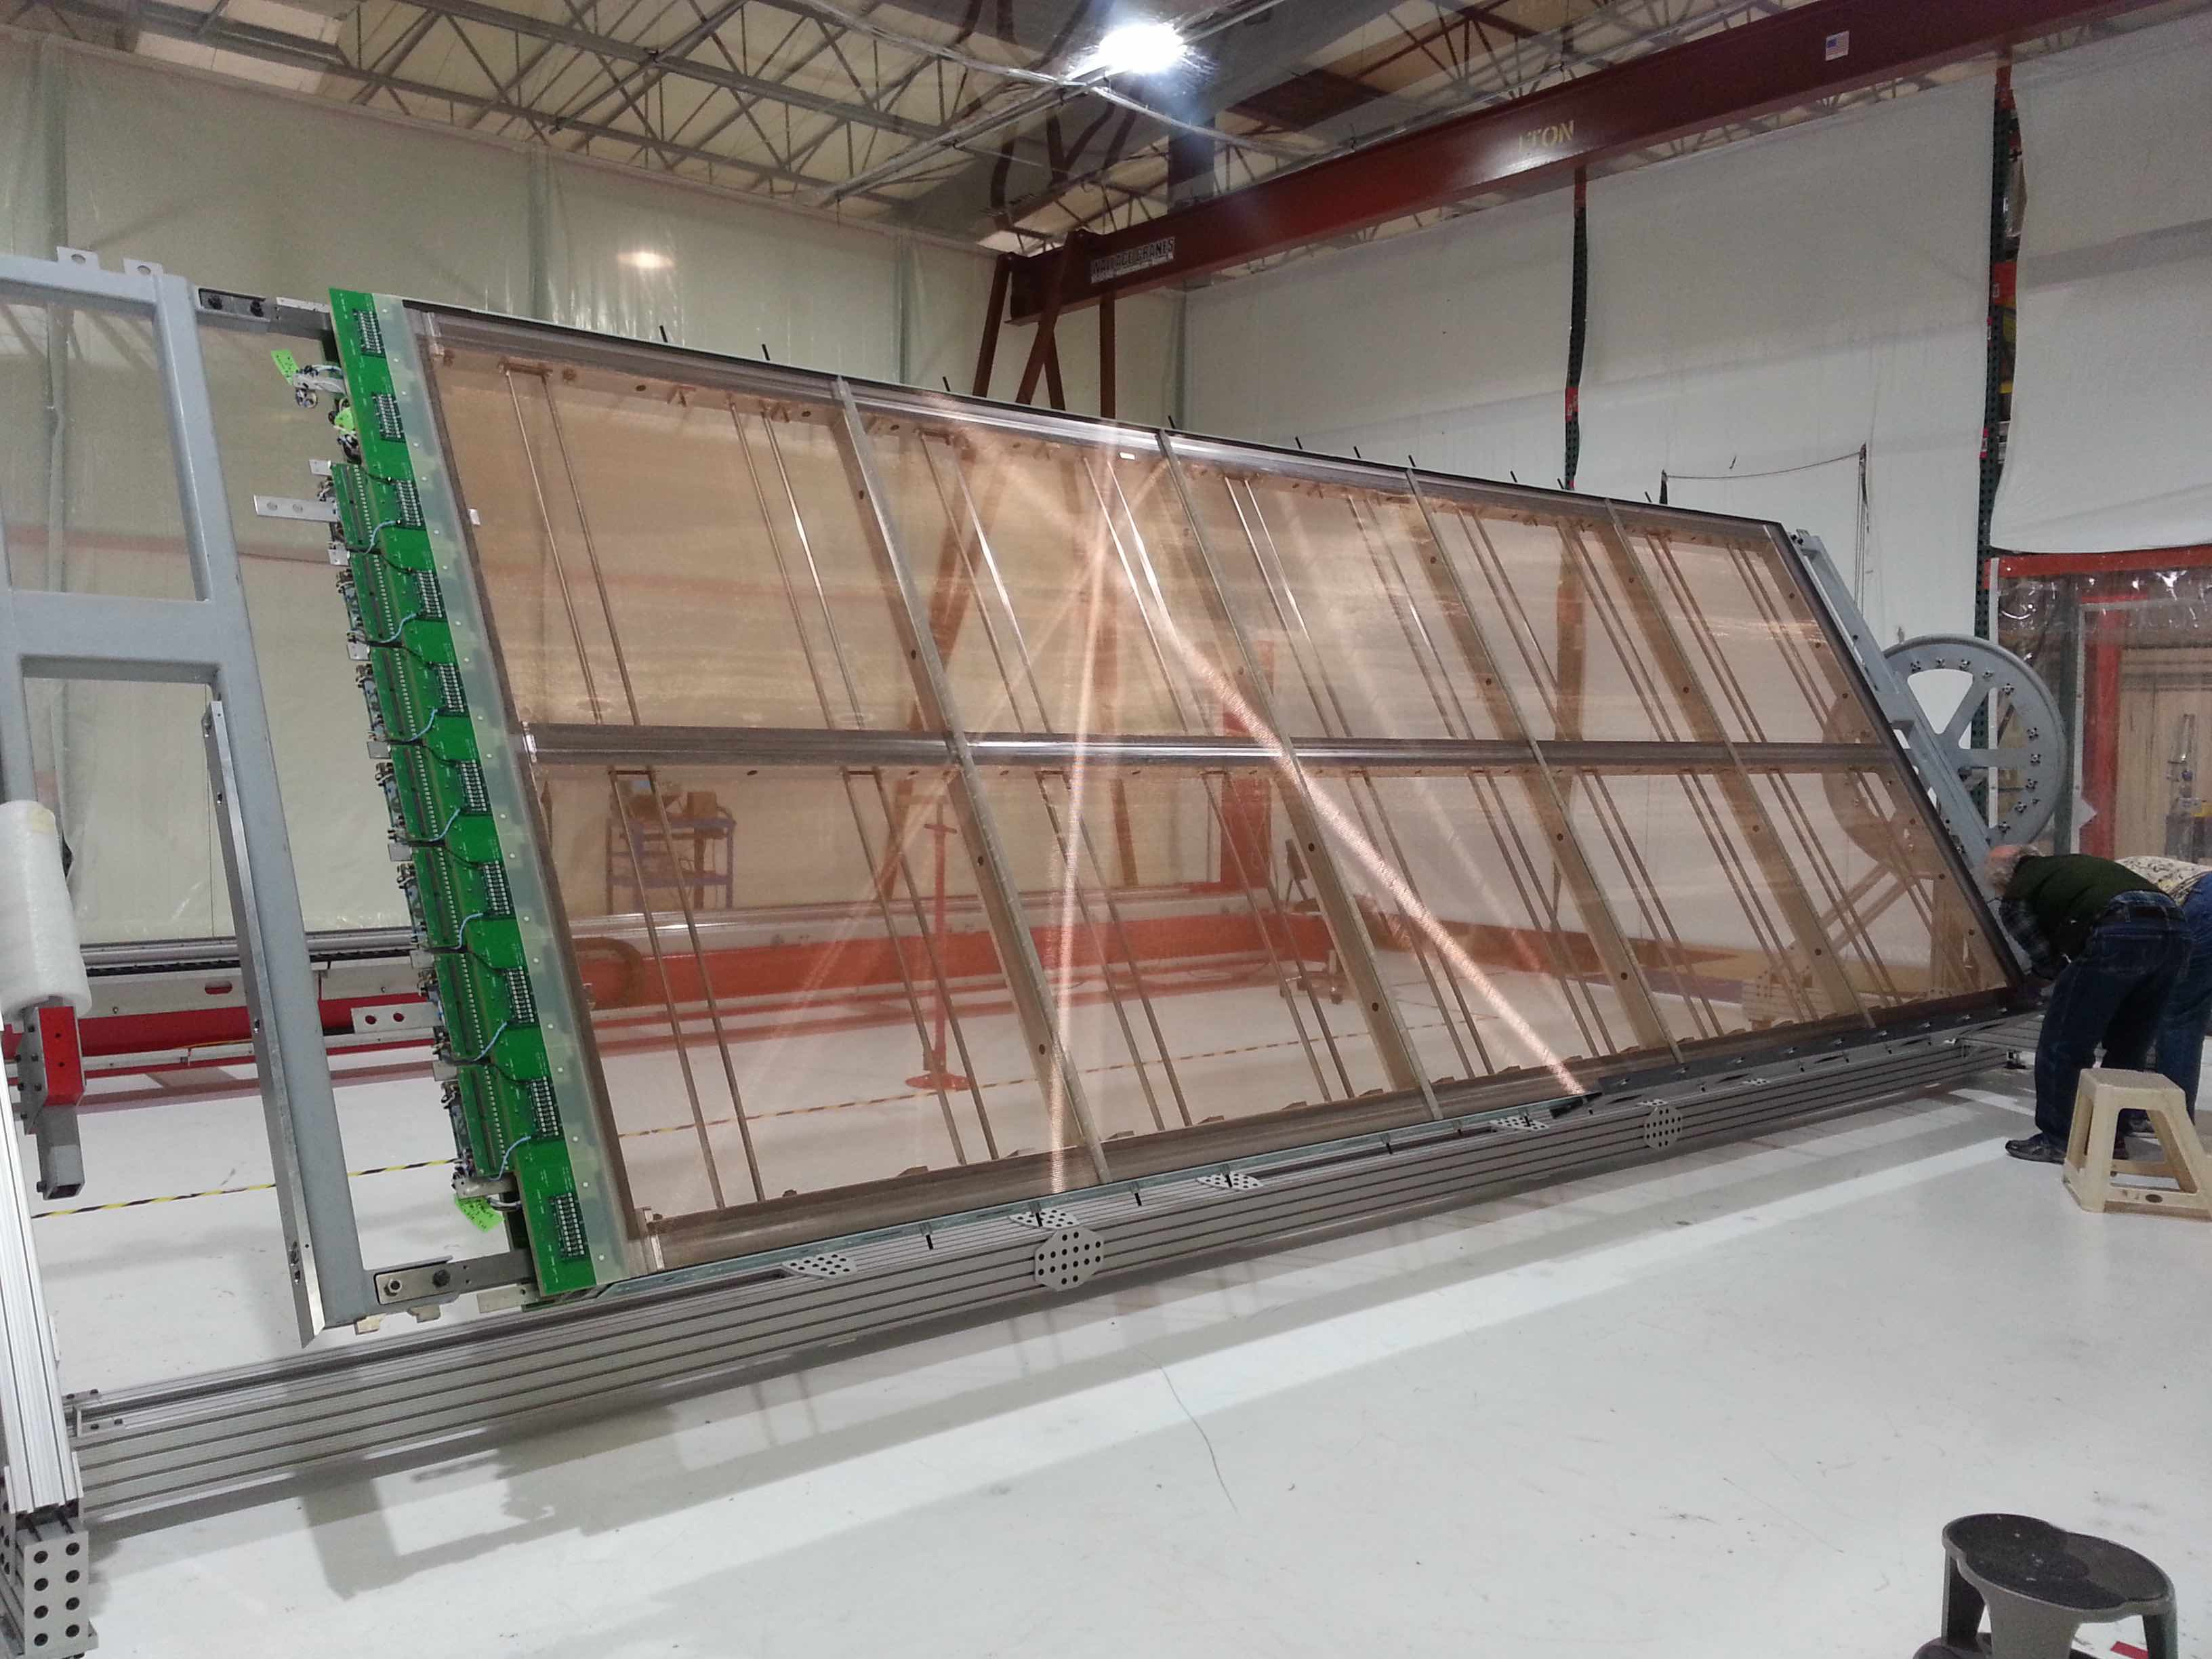
\includegraphics[width=0.9\textwidth,trim=20mm 80mm 0mm 60mm,clip]{apa-photo-complete.jpg}} 
\end{dunefigure}